\chapter{Methods}
\label{cha:methods}

This chapter describes the application of theory shown in Chapter~\ref{cha:theory} applied to the pre-processed data described in Chapter~\ref{cha:data}. For further details regarding coding and implementation, the reader is referred to this work's \href{https://github.com/cosmourao/thesis}{\textcolor{blue}{repository}}.

In general, the use of Scikit-Learn's \texttt{pipeline} class alongside linear models made analysis straightforward. Additionally, Scikit-Learn's \texttt{GridSearchCV} allowed for a faster evaluation of different hyperparameters such as number of components and shrinkage factor.

Throughout all methods, training, test and validation sets were split using \texttt{train\_test\_split}. Out of all 1500 exposures, 1200 (80\%) were assigned to the training set and 300 (20\%) to the validation set. The test set is embedded in the training set, as k-fold cross-validation is used. A fixed random seed of 42 was set to ensure reproducibility of results. 

For reasons that will become clear in Chapter~\ref{cha:discussion} - Discussions, regression analysis was done with two sets of predictor variables: first with all features, i.e. slopes and averages for each exposure, and second with only averages for unique mixtures (averaged features).

\section{\acrlong{ols}}
\label{sec:met-ols}

Here treated as a baseline, \acrshort{ols} is fit using \texttt{LinearRegression} then evaluated using the validation set.

\section{\acrlong{pcr}}
\label{sec:met-pcr}

First, a \acrshort{pca} was conducted via Scikit-Learn's \texttt{PCA}. With that, cumulative variance and score plots were made in an attempt of better visualizing and understanding the data.

Following that, a linear regression on the \acrshort{pc}s was made. The number of components to use in it was found via \acrshort{cv} with \acrshort{rmse} as the scoring function. After training, the model was evaluated in a held-out validation set and a actual vs. predicted plot was constructed.

\section{\acrlong{plsr}}
\label{sec:met-plsr}

Here, a similar procedure to Section~\ref{sec:met-pcr} was conducted. Initially, \acrshort{pls} components were extracted via Scikit-learn's \texttt{PLSRegression} and some informative plots were made: cumulative explained variance (for both predictors $\mathbf{X}$ and response $\mathbf{Y}$), as well as score plots for the first two \acrshort{pls} components in an attempt to better visualize the data. The regression model was trained with the ideal number of components given by \acrshort{cv} and later evaluated in the held-out validation set.

\section{Ridge Regression}
\label{sec:met-ridge}

Once again, cross-validation was use to select the amount of shrinkage, i.e. $\lambda$. After setting $\lambda$, analysis proceeded as usual: fitting the regression line via \texttt{Ridge} to training data and evaluating it using the validation set.

\section{Averaging features}
\label{sec:met-avg}

In efforts to further analyze the data, the previous 1500 observations are averaged by unique mixtures, i.e. for each mixture, the features are averaged from its twelve exposures, yielding 125 observations. Figure~\ref{fig:averaging-process} clarifies this further.

\begin{figure}[h]
	\centering
	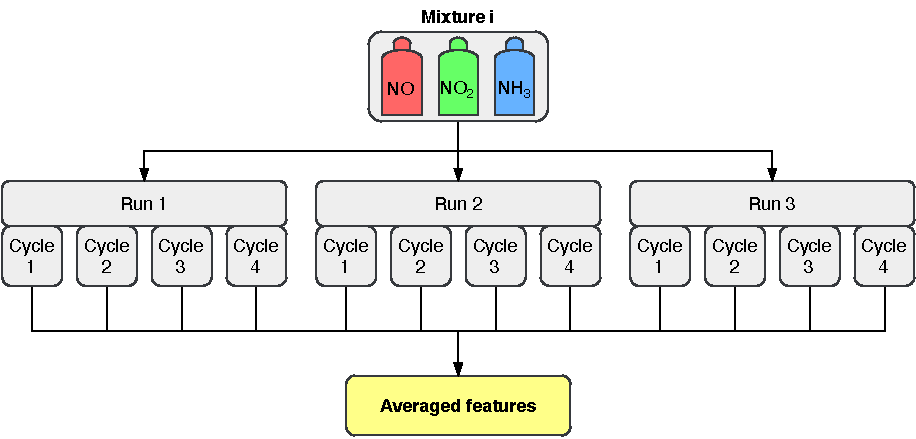
\includegraphics[width=1\textwidth]{../figures/averaging-process.pdf}
	\caption{A visualization of the feature averaging process.}
	\label{fig:averaging-process}
\end{figure}


